\documentclass{article}

% Required packages (merged from hw5_template.tex and hw6_questions.tex)
\usepackage{amssymb}
\usepackage{amsmath}
\usepackage{graphicx}
\usepackage{geometry}
\usepackage{tikz}
\usepackage{array}
\usepackage{booktabs}
\usepackage{enumitem}
\usepackage{listings}
\usepackage{xcolor}
\usepackage{fancyhdr}
\usepackage{float}
\usepackage{subcaption}
\usepackage{comment}
\usepackage{algorithm}
\usepackage{algpseudocode}
\usepackage{caption}
\usepackage{siunitx}
\usepackage{hyperref}
\usetikzlibrary{arrows.meta, positioning} % Required for hw6 diagrams

% Set page geometry
\geometry{a4paper, margin=1in}

% Configure listings for Python
\lstset{
  language=Python,
  basicstyle=\ttfamily\footnotesize,
  numbers=left,
  numberstyle=\tiny\color{gray},
  frame=single,
  breaklines=true,
  breakatwhitespace=true,
  captionpos=b,
  tabsize=4,
  showspaces=false,
  showstringspaces=false,
  showtabs=false,
  commentstyle=\color{gray}\textit,
  keywordstyle=\color{blue}\bfseries,
  stringstyle=\color{red}
}

\begin{document}

\pagestyle{fancy}
\chead{DSC 257: Unsupervised Learning (Fall 2025)}
\lhead{Homework 6}
\rhead{Randall Rogers}

%------------------
% Solution for 1(a)
%------------------
\subsection*{Solution 1}
\noindent\rule{\textwidth}{0.4pt}\\
\subsubsection*{Solution 1 (a)}
The probability density function (PDF) for a $d$-dimensional multivariate Gaussian distribution $N(\mu, \Sigma)$ is:
$$ f(x) = \frac{1}{(2\pi)^{d/2} |\Sigma|^{1/2}} \exp\left( -\frac{1}{2} (x - \mu)^\top \Sigma^{-1} (x - \mu) \right) $$
Given a spherical Gaussian $N(0, I_d)$:
$$\mu = 0 \quad \text{ and }\quad \Sigma = I_d \rightarrow (\text{definition: }N(\mu, \Sigma))$$
The determinant of any identity matrix is $1$, and inverse of an identity matrix is itself:
$$|\Sigma| = |I_d| = 1 \quad \text{ and }\quad \Sigma^{-1} = I_d^{-1} = I_d$$
Now, substitute $\mu$, $\Sigma$, and $|\Sigma|$ into the PDF formula:
\begin{align*}
    f(x) &= \frac{1}{(2\pi)^{d/2} |\Sigma|^{1/2}} \exp\left( -\frac{1}{2} (x - \mu)^\top \Sigma^{-1} (x - \mu) \right) \\
    &= \frac{1}{(2\pi)^{d/2} (1)^{1/2}} \exp\left( -\frac{1}{2} (x - \mathbf{0})^\top I_d (x - \mathbf{0}) \right) \\
    &= \frac{1}{(2\pi)^{d/2}} \exp\left( -\frac{1}{2} x^\top x \right) \\
    &= (2\pi)^{-d/2} \exp\left( -\frac{1}{2} \|x\|^2 \right)
\end{align*}
Next, simplify the expression by taking natural log such that $L(x)=\ln(f(x))$:
\begin{align*}
    L(x) &= \ln\left((2\pi)^{-d/2} \exp\left( -\frac{1}{2} \|x\|^2 \right)\right) \\
    &= \ln\left((2\pi)^{-d/2}\right) + \ln\left(\exp\left( -\frac{1}{2} \|x\|^2 \right)\right) \\
    &= \ln\left((2\pi)^{-d/2}\right) - \frac{1}{2} \|x\|^2  
\end{align*}
By inspection the maximum of $L(x)$ is achived at the mean, $x = 0$.
Hence, the maximum density is:
$$(2\pi)^{-d/2}$$

\subsubsection*{\normalfont}{$\therefore$ The maximum density for a spherical Gaussian $N(0, I_d)$ is $(2\pi)^{-d/2}$, and the point is achieved at $x = 0$}

\noindent\rule{\textwidth}{0.4pt}\\

\newpage

%------------------
% Solution for 1(b)
%------------------
\subsection*{Solution 1}
\noindent\rule{\textwidth}{0.4pt}\\
\subsubsection*{Solution 1 (b)}
From \textit{part (a)}, the maximum density is:
$$f_{\text{max}} = (2\pi)^{-d/2}$$
Consider the limit of the density as $d$ approaches infinity:
$$ \lim_{d \to \infty} (2\pi)^{-d/2} = 0 $$

\subsubsection*{\normalfont}{$\therefore$ The maximum density approaches $0$ as $d$ grows.}

\noindent\rule{\textwidth}{0.4pt}\\

\newpage

%------------------
% Solution for 2(a)
%------------------
\subsection*{Solution 2}
\noindent\rule{\textwidth}{0.4pt}\\
\subsubsection*{Solution 2 (a)}
\subsubsection*{Python Code: d=10}
\begin{lstlisting}
import numpy as np
import matplotlib.pyplot as plt

# set dimension and number of samples
d = 10
num_samples = 10000
np.random.seed(42) 

# get 10000 points from N(0, I_d)
samples = np.random.normal(0, 1, size=(num_samples, d))

# calc the squared L2 norm for each point
squared_lengths_d10 = np.sum(samples**2, axis=1)

# calculate mean
sample_mean_d10 = np.mean(squared_lengths_d10)
print(f"Dimension (d): {d}")
print(f"Sample Mean of ||X||^2: {sample_mean_d10:.4f}")

# plot the histogram
plt.figure(figsize=(10, 6))
plt.hist(squared_lengths_d10, bins=50, color='skyblue', edgecolor='black', alpha=0.7, density=True,label=f'Histogram of {num_samples} samples')
plt.axvline(d, color='red', linestyle='--', linewidth=2, 
            label=f'Theoretical Mean (d = {d}): $E[||X||^2]$')
plt.axvline(sample_mean_d10, color='blue', linestyle=':', linewidth=2, 
            label=f'Sample Mean = {sample_mean_d10:.4f}')
# set plot args and save
plt.title('Histogram of Squared Lengths for $N(0, I_{10})$', fontsize=14)
plt.xlabel('Squared Length $||X||^2$', fontsize=12)
plt.ylabel('Density', fontsize=12)
plt.legend()
plt.grid(True, linestyle='--', alpha=0.5)
plt.savefig('histogram_d10.png', dpi=150, bbox_inches='tight')
\end{lstlisting}

\newpage
%------------------
% Solution for 2(a)
%------------------
\subsection*{Solution 2}
\noindent\rule{\textwidth}{0.4pt}\\
\subsubsection*{Solution 2 (a)}
\subsubsection*{Plot}
\begin{figure}[h]
  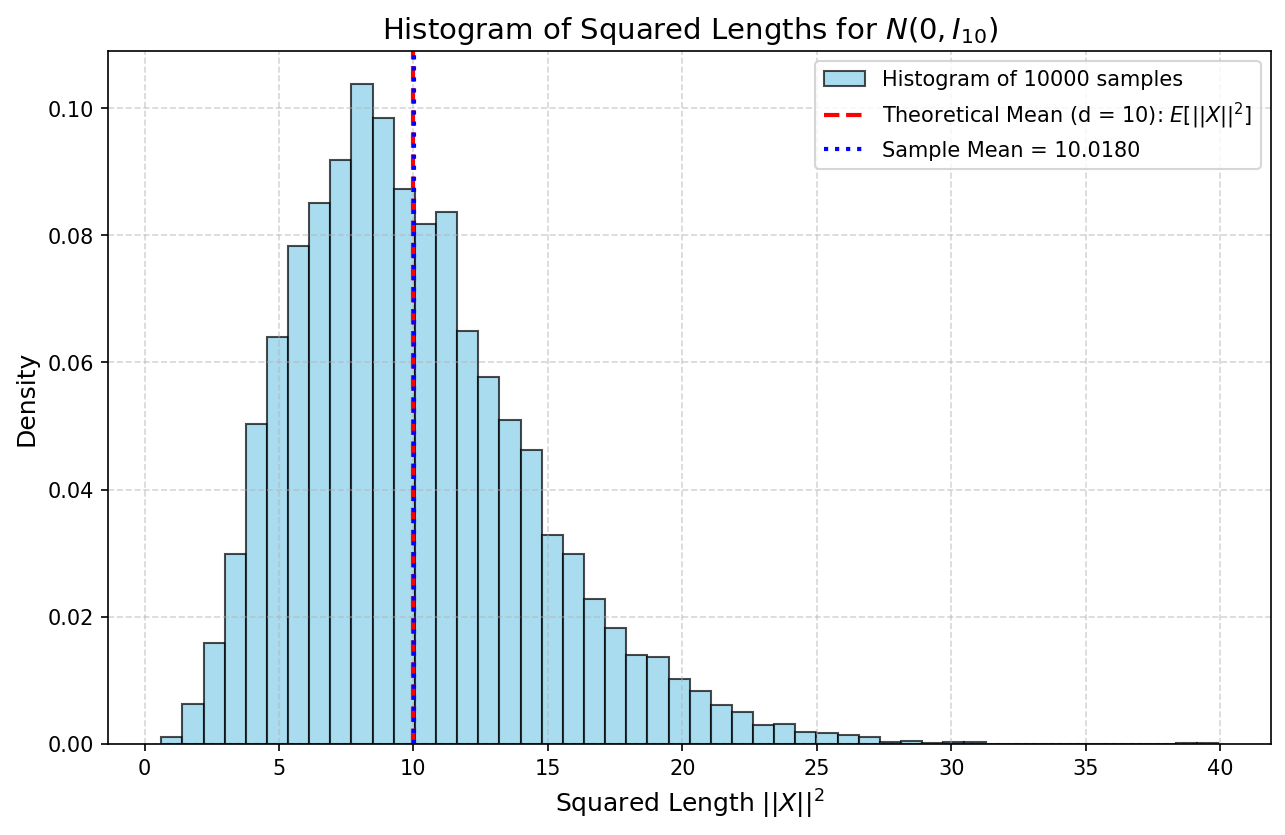
\includegraphics[width=\textwidth]{histogram_d10.png}
  \caption{Histogram of squared lengths for d=10.}
\end{figure}

\subsubsection*{\normalfont}{$\therefore$ The typical (squared) length is approximately 10}

\noindent\rule{\textwidth}{0.4pt}\\

\newpage

%------------------
% Solution for 2(b)
%------------------
\subsection*{Solution 2}
\noindent\rule{\textwidth}{0.4pt}\\
\subsubsection*{Solution 2 (b)}
\subsubsection*{Python Code: d=100}
\begin{lstlisting}
import numpy as np
import matplotlib.pyplot as plt

# set dimension and number of samples
d = 100
num_samples = 10000
np.random.seed(42) 

# get 10000 points from N(0, I_d)
samples = np.random.normal(0, 1, size=(num_samples, d))

# calc the squared L2 norm for each point
squared_lengths_d100 = np.sum(samples**2, axis=1)

# calculate mean
sample_mean_d100 = np.mean(squared_lengths_d100)
print(f"Dimension (d): {d}")
print(f"Sample Mean of ||X||^2: {sample_mean_d100:.4f}")

# plot the histogram
plt.figure(figsize=(10, 6))
plt.hist(squared_lengths_d100, bins=50, color='skyblue', edgecolor='black', alpha=0.7, density=True,label=f'Histogram of {num_samples} samples')
plt.axvline(d, color='red', linestyle='--', linewidth=2, 
            label=f'Theoretical Mean (d = {d}): $E[||X||^2]$')
plt.axvline(sample_mean_d100, color='blue', linestyle=':', linewidth=2, 
            label=f'Sample Mean = {sample_mean_d100:.4f}')
# set plot args and save
plt.title('Histogram of Squared Lengths for $N(0, I_{100})$', fontsize=14)
plt.xlabel('Squared Length $||X||^2$', fontsize=12)
plt.ylabel('Density', fontsize=12)
plt.legend()
plt.grid(True, linestyle='--', alpha=0.5)
plt.savefig('histogram_d100.png', dpi=150, bbox_inches='tight')
\end{lstlisting}

\newpage
\subsection*{Solution 2}
\noindent\rule{\textwidth}{0.4pt}\\
\subsubsection*{Solution 2 (b)}
\subsubsection*{Plot}
\begin{figure}[h]
  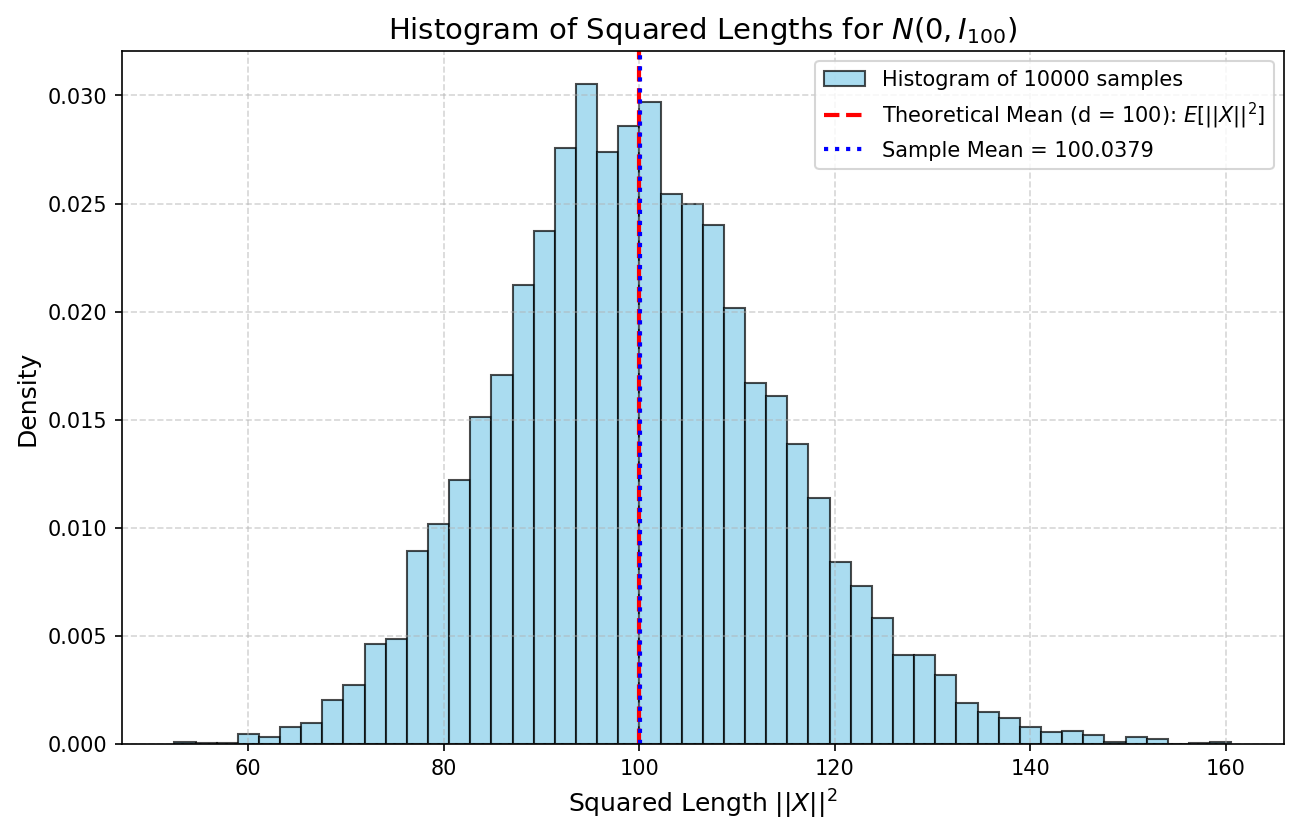
\includegraphics[width=\textwidth]{histogram_d100.png}
  \caption{Histogram of squared lengths for d=100.}
\end{figure}

\subsubsection*{Calculate Concentration}
To determine if the distribution is more concentrated, we must compare its relative spread. This is measured using the coefficient of variation or $CV$, which is defined as:
$$CV = \frac{\sigma}{\mu} \quad \text{ where } \quad \mu=d \text{ ,  } \sigma = \sqrt{2d}$$
For, $d=10$ and $d=100$, the coefficient of variation is:
$$CV_{10} = \frac{\sqrt{20}}{10} \approx 0.447\quad \text{ and }\quad CV_{100} = \frac{\sqrt{200}}{100} \approx 0.141$$
Hence, $CV_{100} < CV_{10}$ 

\subsubsection*{\normalfont}{$\therefore$ the distribution for $d=100$ is more concentrated than the distribution for $d=10$}

\noindent\rule{\textwidth}{0.4pt}\\

\newpage

%------------------
% Solution for 3
%------------------
\subsection*{Solution 3}
\noindent\rule{\textwidth}{0.4pt}\\

Let $X \sim N(\mu, \Sigma)$ where:
$$ \mu = \begin{bmatrix}1 \\ 2\end{bmatrix} \quad \quad \Sigma = \begin{bmatrix}2 & 0 \\ 0 & 4\end{bmatrix} \quad \quad v = \frac{1}{\sqrt{2}}\begin{bmatrix}1 \\ 1\end{bmatrix}$$

\begin{enumerate}
    \item Calculate the mean $\mu_Y$:
    \begin{align*}
    \mu_Y &= v^\top\mu \\
          &= \begin{bmatrix}1/\sqrt{2} & 1/\sqrt{2}\end{bmatrix} \begin{bmatrix}1 \\ 2\end{bmatrix} \\
          &= \left(\frac{1}{\sqrt{2}} \cdot 1\right) + \left(\frac{1}{\sqrt{2}} \cdot 2\right) \\
          &= \frac{1}{\sqrt{2}} + \frac{2}{\sqrt{2}} \\
          &= \frac{3}{\sqrt{2}}
    \end{align*}
    \item Calculate the variance $\sigma_Y^2$:
    \begin{align*}
        \sigma_Y^2 &= v^\top\Sigma v \\
        &= \begin{bmatrix}1/\sqrt{2} & 1/\sqrt{2}\end{bmatrix} \begin{bmatrix}2 & 0 \\ 0 & 4\end{bmatrix} \begin{bmatrix}1/\sqrt{2} \\ 1/\sqrt{2}\end{bmatrix} \\
        &= \begin{bmatrix}1/\sqrt{2} & 1/\sqrt{2}\end{bmatrix} \begin{bmatrix} 2 \cdot (1/\sqrt{2}) + 0 \\ 0 + 4 \cdot (1/\sqrt{2}) \end{bmatrix} \\
        &= \begin{bmatrix}1/\sqrt{2} & 1/\sqrt{2}\end{bmatrix} \begin{bmatrix} 2/\sqrt{2} \\ 4/\sqrt{2} \end{bmatrix} \\
        &= \left(\frac{1}{\sqrt{2}} \cdot \frac{2}{\sqrt{2}}\right) + \left(\frac{1}{\sqrt{2}} \cdot \frac{4}{\sqrt{2}}\right) \\
        &= \frac{2}{2} + \frac{4}{2} \\
        &= 1 + 2 = 3
    \end{align*}
\end{enumerate}

\subsubsection*{\normalfont}{$\therefore$ The distribution of the projection is $N\left(\frac{3}{\sqrt{2}}, 3\right)$}

\noindent\rule{\textwidth}{0.4pt}\\

\newpage

%------------------
% Solution for 4(a)
%------------------
\subsection*{Solution 4}
\noindent\rule{\textwidth}{0.4pt}\\
\subsubsection*{Solution 4 (a)}
Let, $X = \begin{bmatrix} X_1 \\ X_2 \\ X_3 \end{bmatrix} \sim N(\mu, \Sigma)$, where:
$$ \mu = \begin{bmatrix} 0 \\ 0 \\ 0 \end{bmatrix} \quad \text{and} \quad \Sigma = \begin{bmatrix} 6 & 3 & 1 \\ 3 & 9 & 0 \\ 1 & 0 & 2 \end{bmatrix} $$
Since the distribution for $X_3$ is a 1D Gaussian $N(\mu_3, \sigma_{3}^2)$, we can just lookup the mean and variance of $X_3$ from the given covariance matrix. Note, $\sigma_{3}^2 = \sigma_{(3,3)}^2$
$$\mu = \begin{bmatrix} \mu_1 \\ \mu_2 \\ \mu_3 \end{bmatrix} = \begin{bmatrix} 0 \\ 0 \\ 0 \end{bmatrix} \rightarrow \mu_3 = 0 $$
$$\Sigma = \begin{bmatrix} \sigma_{(1,1)}^2 & \sigma_{(1,2)}^2 & \sigma_{(1,3)}^2 \\ \sigma_{(2,1)}^2 & \sigma_{(2,2)}^2 & \sigma_{(2,3)}^2 \\ \sigma_{(3,1)}^2 & \sigma_{(3,2)}^2 & \sigma_{(3,3)}^2 \end{bmatrix} = \begin{bmatrix} 6 & 3 & 1 \\ 3 & 9 & 0 \\ 1 & 0 & 2 \end{bmatrix} \rightarrow \sigma_{(3,3)}^2 = 2$$ 

\subsubsection*{\normalfont}{$\therefore$ The distribution of $X_3$ is:} 
$$N(0, 2)$$


\noindent\rule{\textwidth}{0.4pt}\\

\newpage

%------------------
% Solution for 4(b)
%------------------
\subsection*{Solution 4}
\noindent\rule{\textwidth}{0.4pt}\\
\subsubsection*{Solution 4 (b)}
Let, $X = \begin{bmatrix} X_1 \\ X_2 \\ X_3 \end{bmatrix} \sim N(\mu, \Sigma)$, where:
$$ \mu = \begin{bmatrix} 0 \\ 0 \\ 0 \end{bmatrix} \quad \text{and} \quad \Sigma = \begin{bmatrix} 6 & 3 & 1 \\ 3 & 9 & 0 \\ 1 & 0 & 2 \end{bmatrix} $$
Since we want the joint distribution for $X_1$ and $X_2$, it follows that it is a 2D Gaussian $N(\mu_{1,2}, \Sigma_{1,2})$ or:
$$N\left(\begin{bmatrix} \mu_1 \\ \mu_2 \end{bmatrix}\text{ ,  }\begin{bmatrix} \sigma_{1,1}^2 & \sigma_{1,2}^2 \\ \sigma_{2,1}^2 & \sigma_{2,2}^2 \end{bmatrix}\right)$$
It follows that,
$$\mu = \begin{bmatrix} \mu_1 \\ \mu_2 \\ \mu_3 \end{bmatrix} = \begin{bmatrix} 0 \\ 0 \\ 0 \end{bmatrix} \rightarrow \mu_{1,2} = \mu_{1,2} = \begin{bmatrix} \mu_1 \\ \mu_2 \end{bmatrix} = \begin{bmatrix} 0 \\ 0 \end{bmatrix}$$
$$\Sigma = \begin{bmatrix} \sigma_{(1,1)}^2 & \sigma_{(1,2)}^2 & \sigma_{(1,3)}^2 \\ \sigma_{(2,1)}^2 & \sigma_{(2,2)}^2 & \sigma_{(2,3)}^2 \\ \sigma_{(3,1)}^2 & \sigma_{(3,2)}^2 & \sigma_{(3,3)}^2 \end{bmatrix} = \begin{bmatrix} 6 & 3 & 1 \\ 3 & 9 & 0 \\ 1 & 0 & 2 \end{bmatrix} \rightarrow \Sigma_{1,2} = \begin{bmatrix} \sigma_{1,1}^2 & \sigma_{1,2}^2 \\ \sigma_{2,1}^2 & \sigma_{2,2}^2 \end{bmatrix} = \begin{bmatrix} 6 & 3 \\ 3 & 9 \end{bmatrix}$$ 

\subsubsection*{\normalfont}{$\therefore$ The joint distribution of $X_1$, $X_2$ is:
$$N\left(\begin{bmatrix} 0 \\ 0 \end{bmatrix}, \begin{bmatrix} 6 & 3 \\ 3 & 9 \end{bmatrix}\right)$$}

\noindent\rule{\textwidth}{0.4pt}\\

\newpage

%------------------
% Solution for 4(c)
%------------------
\subsection*{Solution 4}
\noindent\rule{\textwidth}{0.4pt}\\
\subsubsection*{Solution 4 (c)}
Let, $X = \begin{bmatrix} X_1 \\ X_2 \\ X_3 \end{bmatrix} \sim N(\mu, \Sigma)$, where:
$$ \mu = \begin{bmatrix} 0 \\ 0 \\ 0 \end{bmatrix} \quad \text{and} \quad \Sigma = \begin{bmatrix} 6 & 3 & 1 \\ 3 & 9 & 0 \\ 1 & 0 & 2 \end{bmatrix} $$
We need to find the conditional distribution of $X_1 \mid (X_2, X_3)$.
Let $X_a = X_1$ and $X_b = \begin{bmatrix} X_2 \\ X_3 \end{bmatrix}$. We observe $x_b = \begin{bmatrix} 2 \\ 1 \end{bmatrix}$.
Now, partition the mean vector $\mu$ and covariance matrix $\Sigma$:
$$ \mu = \begin{bmatrix} \mu_a \\ \mu_b \end{bmatrix} = \begin{bmatrix} 0 \\ \hline 0 \\ 0 \end{bmatrix} \quad \text{ and }\quad \Sigma = \begin{bmatrix} \Sigma_{aa} & \Sigma_{ab} \\ \Sigma_{ba} & \Sigma_{bb} \end{bmatrix} = \left[ \begin{array}{c|cc} 6 & 3 & 1 \\ \hline 3 & 9 & 0 \\ 1 & 0 & 2 \end{array} \right] $$
From this, we identify the blocks:
$$\mu_a = 0 \qquad \mu_b = \begin{bmatrix} 0 \\ 0 \end{bmatrix} \qquad \Sigma_{aa} = 6 \qquad \Sigma_{ab} = \begin{bmatrix} 3 & 1 \end{bmatrix} \qquad \Sigma_{ba} = \begin{bmatrix} 3 \\ 1 \end{bmatrix} \qquad \Sigma_{bb} = \begin{bmatrix} 9 & 0 \\ 0 & 2 \end{bmatrix}$$
The conditional distribution $X_a \mid X_b = x_b$ is also Gaussian, $N(\mu_{a|b}, \Sigma_{a|b})$, where:
$$\mu_{a|b} = \mu_a + \Sigma_{ab} \Sigma_{bb}^{-1} (x_b - \mu_b) \quad \text{ and } \quad \Sigma_{a|b} = \Sigma_{aa} - \Sigma_{ab} \Sigma_{bb}^{-1} \Sigma_{ba}$$
\begin{enumerate}
    \item Compute $\Sigma_{bb}^{-1}$: \textit{Since $\Sigma_{bb}$ is diagonal, its inverse is the inverse of its diagonal elements:}
    $$ \Sigma_{bb}^{-1} = \begin{bmatrix} 9 & 0 \\ 0 & 2 \end{bmatrix}^{-1} = \begin{bmatrix} 1/9 & 0 \\ 0 & 1/2 \end{bmatrix} $$
    \item Compute the conditional mean $\mu_{a|b}$:
    $$\mu_{a|b} = \mu_a + \Sigma_{ab} \Sigma_{bb}^{-1} (x_b - \mu_b) = 0 + \begin{bmatrix} 3 & 1 \end{bmatrix} \begin{bmatrix} 1/9 & 0 \\ 0 & 1/2 \end{bmatrix} \left( \begin{bmatrix} 2 \\ 1 \end{bmatrix} - \begin{bmatrix} 0 \\ 0 \end{bmatrix} \right) = \begin{bmatrix} 1/3 & 1/2 \end{bmatrix} \begin{bmatrix} 2 \\ 1 \end{bmatrix} = \frac{7}{6}$$
    \item Compute the conditional variance $\Sigma_{a|b}$:
    $$\Sigma_{a|b} = 6 - \begin{bmatrix} 3 & 1 \end{bmatrix} \begin{bmatrix} 1/9 & 0 \\ 0 & 1/2 \end{bmatrix} \begin{bmatrix} 3 \\ 1 \end{bmatrix} = 6 - \begin{bmatrix} 1/3 & 1/2 \end{bmatrix} \begin{bmatrix} 3 \\ 1 \end{bmatrix} = 6 - \left( \left(\frac{1}{3} \cdot 3\right) + \left(\frac{1}{2} \cdot 1\right) \right) = \frac{9}{2}$$
\end{enumerate}
\subsubsection*{\normalfont}{$\therefore$ The resulting conditional distribution of $X_1$ is:}
$$N\left(\frac{7}{6}, \frac{9}{2}\right)$$

\noindent\rule{\textwidth}{0.4pt}\\

\newpage

%------------------
% Solution for 5(a)
%------------------
\subsection*{Solution 5}
\noindent\rule{\textwidth}{0.4pt}
\subsubsection*{Solution 5 (a)}
A Gaussian Process is defined as a (potentially infinite) collection of random variables, any finite subset of which has a joint multivariate Gaussian distribution.
The finite subset in this example is the $93$ training and $11$ test points, which we can express as:
$$\begin{bmatrix} y_{\text{tr}} \\ y_{\text{te}} \end{bmatrix}$$
\subsubsection*{\normalfont}{$\therefore$ By the definition of a Gaussian Process, this finite collection of 104 random variables must have a joint multivariate Gaussian distribution}

\noindent\rule{\textwidth}{0.4pt}\\

\newpage

%------------------
% Solution for 5(b)
%------------------
\subsection*{Solution 5}
\noindent\rule{\textwidth}{0.4pt}\\
\subsubsection*{Solution 5 (b)}
\subsubsection*{Python Code: Posterior Mean and MSE}
\begin{lstlisting}[language=Python]
import numpy as np
import pandas as pd
from scipy.spatial.distance import cdist

def load_data(filename):
    data = pd.read_csv(filename, header=None)
    data.columns = ['latitude', 'longitude', 'temperature']
    X = data[['latitude', 'longitude']].values
    y = data['temperature'].values
    return X, y

def kernel(X1, X2, sigma=1.5):
    # cdist computes the Euclidean distance between all pairs
    dists = cdist(X1, X2, metric='euclidean')
    return np.exp(-dists / sigma)

# load data
X_tr, y_tr = load_data('gptrain.csv')
X_te, y_te = load_data('gptest.csv')
# set model parameters
SIGMA = 1.5
MEAN_VAL = 20.0
JITTER = 1e-6 
# calc mean vectors 
m_tr = np.full(y_tr.shape, MEAN_VAL)
m_te = np.full(y_te.shape, MEAN_VAL)
# calc kernel Matrices 
K_tr = kernel(X_tr, X_tr, sigma=SIGMA)
K_tr_stable = K_tr + np.eye(K_tr.shape[0]) * JITTER
K_te_tr = kernel(X_te, X_tr, sigma=SIGMA)
# calc GP posterior mean
alpha = np.linalg.solve(K_tr_stable, y_tr - m_tr)
mu_post = m_te + K_te_tr @ alpha
# calc GP MSE 
mse_gp = np.mean((mu_post - y_te)**2)
print(f"\nGP Posterior Mean: {mu_post}")
print(f"Actual Test Values: {y_te}")
print(f"GP Mean Squared Error (MSE): {mse_gp:.6f}")
# calc baseline MSE
baseline_pred = np.mean(y_tr)
mse_baseline = np.mean((baseline_pred - y_te)**2)
print(f"Baseline (Average Training) Prediction: {baseline_pred:.6f}")
print(f"Baseline Mean Squared Error (MSE): {mse_baseline:.6f}")
\end{lstlisting}

\subsubsection*{Code Output}
\begin{verbatim}
GP Posterior Mean: [18.11251828 21.97092191 21.21172958 15.76871264 20.23993114 21.2800907
 16.96205493 21.84549615 20.6904639  20.2495184  18.08471762]
Actual Test Values: [16.3 22.1 20.4 14.8 19.7 20.5 18.4 19.1 22.6 22.9 17.4]
GP Mean Squared Error (MSE): 2.413174
Baseline (Average Training) Prediction: 18.970968
Baseline Mean Squared Error (MSE): 6.422837
\end{verbatim}

\subsubsection*{\normalfont}{$\therefore$ The Mean Squared Error of the Gaussian Process is 2.413174. The Mean Squared Error from predicting the average of the training data is 6.422837.}

\noindent\rule{\textwidth}{0.4pt}\\

\newpage

%------------------
% Solution for 5(c)
%------------------
\subsection*{Solution 5}
\noindent\rule{\textwidth}{0.4pt}\\
\subsubsection*{Solution 5 (c)}
\subsubsection*{Python Code: Grid Predictions and Plots}
\begin{lstlisting}[language=Python]
import numpy as np
import pandas as pd
import matplotlib.pyplot as plt
from scipy.spatial.distance import cdist

def load_data(filename):
    data = pd.read_csv(filename, header=None)
    data.columns = ['latitude', 'longitude', 'temperature']
    X = data[['latitude', 'longitude']].values
    y = data['temperature'].values
    return X, y

def kernel(X1, X2, sigma=1.5):
    dists = cdist(X1, X2, metric='euclidean')
    return np.exp(-dists / sigma)

# load data and set model parameters
X_tr, y_tr = load_data('gptrain.csv')
SIGMA = 1.5
MEAN_VAL = 20.0
JITTER = 1e-6

# pre-compute for posterior
m_tr = np.full(y_tr.shape, MEAN_VAL)
K_tr = kernel(X_tr, X_tr, sigma=SIGMA)
K_tr_stable = K_tr + np.eye(K_tr.shape[0]) * JITTER
alpha = np.linalg.solve(K_tr_stable, y_tr - m_tr)

# create grid (6400 points)
GRID_SIZE = 80 
lat_min, lat_max = X_tr[:, 0].min(), X_tr[:, 0].max()
lon_min, lon_max = X_tr[:, 1].min(), X_tr[:, 1].max()
lat_grid = np.linspace(lat_min, lat_max, GRID_SIZE)
lon_grid = np.linspace(lon_min, lon_max, GRID_SIZE)
LON, LAT = np.meshgrid(lon_grid, lat_grid)

# stack data into (n_grid_points, 2) array
X_grid = np.column_stack([LAT.ravel(), LON.ravel()])
print(f"Created grid with {X_grid.shape[0]} points.")

# calc posterior mean on grid
m_grid = np.full(X_grid.shape[0], MEAN_VAL)
K_grid_tr = kernel(X_grid, X_tr, sigma=SIGMA)
mu_grid = m_grid + K_grid_tr @ alpha
mu_grid_reshaped = mu_grid.reshape(LAT.shape)

# calc posterior standard deviation on grid
K_diag = np.ones(X_grid.shape[0]) 

# use Cholesky decomposition and solve
L = np.linalg.cholesky(K_tr_stable) 
V = np.linalg.solve(L, K_grid_tr.T) 
diag_term = np.sum(V**2, axis=0) 

# calc posterior variance
var_grid = K_diag - diag_term
# Clip at 0 for numerical stability before sqrt
std_grid = np.sqrt(np.maximum(var_grid, 0)) 
std_grid_reshaped = std_grid.reshape(LAT.shape)

# plot results
fig, ax = plt.subplots(1, 2, figsize=(16, 7))
plot_extent = [lon_min, lon_max, lat_min, lat_max]

# plot posterior mean
im1 = ax[0].imshow(mu_grid_reshaped, extent=plot_extent, 
                   origin='lower', aspect='auto', cmap='hot')
ax[0].scatter(X_tr[:, 1], X_tr[:, 0], c='blue', marker='x', label='Training Stations')
ax[0].set_xlabel('Longitude')
ax[0].set_ylabel('Latitude')
ax[0].set_title('GP Posterior Mean Temperature')
ax[0].legend()
fig.colorbar(im1, ax=ax[0], label='Temperature ($\deg$C)')

# plot posterior standard deviation
im2 = ax[1].imshow(std_grid_reshaped, extent=plot_extent, 
                   origin='lower', aspect='auto', cmap='viridis')
ax[1].scatter(X_tr[:, 1], X_tr[:, 0], c='red', marker='x', label='Training Stations')
ax[1].set_xlabel('Longitude')
ax[1].set_ylabel('Latitude')
ax[1].set_title('GP Posterior Standard Deviation')
ax[1].legend()
fig.colorbar(im2, ax=ax[1], label='Std. Deviation ($\deg$C)')

plt.tight_layout()
# Save the figure to be included in the LaTeX document
plt.savefig('gp_predictions.png', dpi=150, bbox_inches='tight')

\end{lstlisting}

\newpage

\subsection*{Solution 5}
\noindent\rule{\textwidth}{0.4pt}\\
\subsubsection*{Solution 5 (c)}
\subsubsection*{Plots}

\begin{figure}[h]
  \centering
  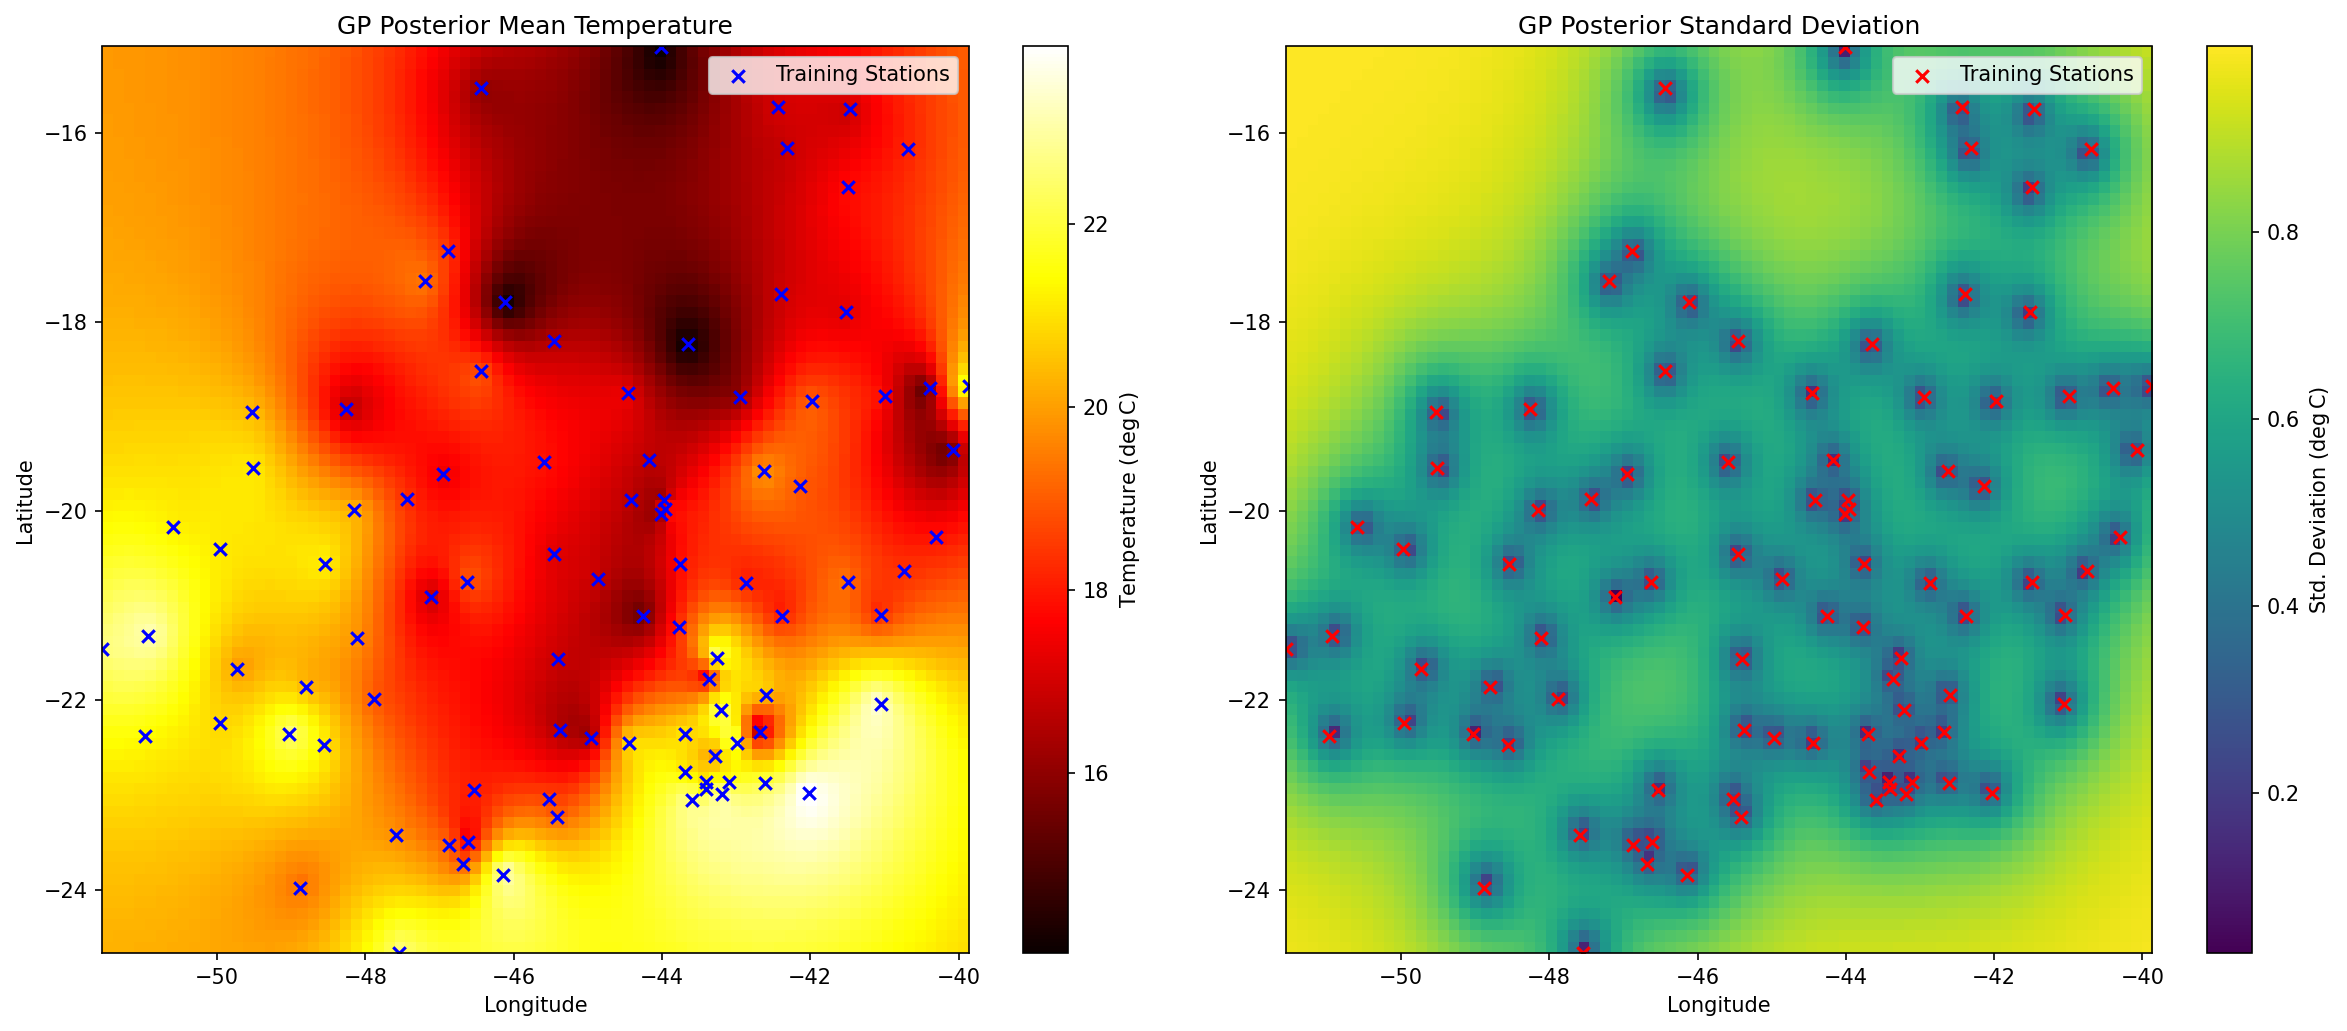
\includegraphics[width=\textwidth]{gp_predictions.png}
  \caption{Posterior mean temperature (left) and posterior standard deviation (right) over the grid. Training station locations are marked with an 'x'.}
\end{figure}

\subsubsection*{Standard Deviation Relationship}
The relationship is clear from the right-hand plot:
The standard deviation of the prediction is lowest at or very close to the locations of the training stations.
As the distance from the nearest training station increases, the standard deviation increases.

\noindent\rule{\textwidth}{0.4pt}\\

\newpage

%------------------
% Solution for 6(a)
%------------------
\subsection*{Solution 6}
\noindent\rule{\textwidth}{0.4pt}\\
\subsubsection*{Solution 6 (a)}
\subsubsection*{Construct Conditional Probability Tables (CPTs)}
\begin{enumerate}
    \item CPT for $F_1$: $P(F_1)$
    \begin{center}
    \begin{tabular}{c c}
    \toprule
    $P(F_1=1)$ & $P(F_1=0)$ \\
    \midrule
    0.5 & 0.5 \\
    \bottomrule
    \end{tabular}
    \end{center}
    \item CPT for $F_2$: $P(F_2)$
    \begin{center}
    \begin{tabular}{c c}
    \toprule
    $P(F_2=1)$ & $P(F_2=0)$ \\
    \midrule
    0.7 & 0.3 \\
    \bottomrule
    \end{tabular}
    \end{center}
    \item CPT for $F_3$: $P(F_3 \mid F_1, F_2)$
    \begin{center}
    \begin{tabular}{c c | c c}
    \toprule
    $F_1$ & $F_2$ & $P(F_3=1)$ & $P(F_3=0)$ \\
    \midrule
    0 & 0 & 0.3 & 0.7 \\
    0 & 1 & 0.8 & 0.2 \\
    1 & 0 & 0.8 & 0.2 \\
    1 & 1 & 0.8 & 0.2 \\
    \bottomrule
    \end{tabular}
    \end{center}
    \item CPT for $F_4$: $P(F_4 \mid F_3)$
    \begin{center}
    \begin{tabular}{c | c c}
    \toprule
    $F_3$ & $P(F_4=1)$ & $P(F_4=0)$ \\
    \midrule
    0 & 0.5 & 0.5 \\
    1 & 0.9 & 0.1 \\
    \bottomrule
    \end{tabular}
    \end{center}
\end{enumerate}

\subsubsection*{\normalfont}{$\therefore$ The Conditional Probability Tables (CPTs) for the model can be seen above}

\noindent\rule{\textwidth}{0.4pt}\\

\newpage
%------------------
% Solution for 6(b)
%------------------
\subsection*{Solution 6}
\noindent\rule{\textwidth}{0.4pt}\\
\subsubsection*{Solution 6 (b)}
Given:
\begin{center}
    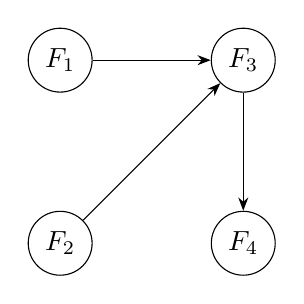
\begin{tikzpicture}[node distance=1.5cm]
        \node[circle, draw] (F1) {$F_1$}; 
        \node[circle, draw, below=of F1] (F2) {$F_2$}; 
        \node[circle, draw, right=of F1] (F3) {$F_3$};
        \node[circle, draw, below=of F3] (F4) {$F_4$};
        \draw[-Stealth] (F1) -- (F3); 
        \draw[-Stealth] (F2) -- (F3); 
        \draw[-Stealth] (F3) -- (F4); 
    \end{tikzpicture}
\end{center}
The joint probability distribution specified by this Bayesian Network is:
$$ P(F_1, F_2, F_3, F_4) = P(F_1) \cdot P(F_2) \cdot P(F_3 \mid F_1, F_2) \cdot P(F_4 \mid F_3) $$
From the tables in \textit{part(a)}:
$$P(F_1=1) = 0.5 \quad P(F_2=1) = 0.7 \quad P(F_3=1 \mid F_1=1, F_2=1) = 0.8 \quad P(F_4=0 \mid F_3=1) = 0.1$$
Now, substitute the values into the equation above for $P(F_1, F_2, F_3, F_4)$:
\begin{align*}
    P(F_1=1, F_2=1, F_3=1, F_4=0) &= P(F_1=1) \times P(F_2=1) \times P(F_3=1 \mid F_1=1, F_2=1) \times P(F_4=0 \mid F_3=1) \\
                                 &= (0.5) \times (0.7) \times (0.8) \times (0.1) \\
                                 &= (0.35) \times (0.08) \\
                                 &= 0.028
\end{align*}

\subsubsection*{\normalfont}{$\therefore$ The probability of the configuration $F_1 = F_2 = F_3 = 1, F_4 = 0$ is $0.028$}

\noindent\rule{\textwidth}{0.4pt}\\

\newpage

%------------------
% Solution for 7
%------------------
\subsection*{Solution 7}
\noindent\rule{\textwidth}{0.4pt}\\
\subsubsection*{Left DAG}
Consider the DAG below:
\begin{center}
    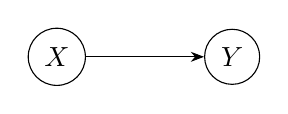
\begin{tikzpicture}[node distance=1.5cm]
        \node[circle, draw] (F1) {$X$}; 
        \node[circle, draw, right=of F1] (F3) {$Y$}; 
        \draw[-Stealth] (F1) -- (F3); 
    \end{tikzpicture}
\end{center}
The rules of Bayesian networks (that a variable is conditioned on its parents), the DAG above implies a factorization of the joint probability as:
    $$P(X,Y) = P(X) \cdot P(Y \mid X)$$
From the chain rule of probability, any joint distribution $P(X,Y)$ can always be written as:
$$P(X)P(Y \mid X)$$
Hence, the factorization required by the Left DAG  for any $P(X,Y)$
\subsubsection*{Right DAG}
Consider the DAG below:
\begin{center}
    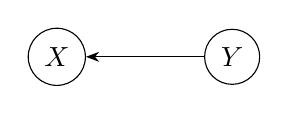
\begin{tikzpicture}[node distance=1.5cm]
        \node[circle, draw] (F1) {$X$}; 
        \node[circle, draw, right=of F1] (F3) {$Y$}; 
        \draw[-Stealth] (F3) -- (F1); 
    \end{tikzpicture}
\end{center}
This DAG implies a factorization of the joint probability as:
$$P(X,Y) = P(Y) \cdot P(X \mid Y)$$
From the chain rule of probability, any joint distribution $P(X,Y)$ can always be written as:
$$P(Y)P(X \mid Y)$$
Hence, the factorization required by the DAG  for any $P(X,Y)$
\subsubsection*{\normalfont}{$\therefore$ Any joint distribution $P(X, Y)$ factors over both the DAGs}

\noindent\rule{\textwidth}{0.4pt}\\

\newpage

%------------------
% Solution for 8(a)
%------------------
\subsection*{Solution 8}
\noindent\rule{\textwidth}{0.4pt}\\
\subsubsection*{Solution 8 (a)}

\subsubsection*{Bayes Net Diagram}
Given:
\begin{itemize}
    \item $G_1$ and $G_2$ are independent.
    \item $D$ depends on $G_1$ and $G_2$.
    \item $P$ depends on $D$.
\end{itemize}

\begin{center}
    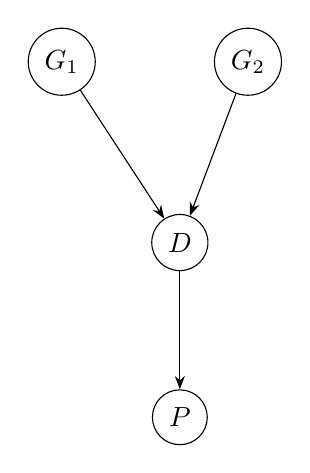
\begin{tikzpicture}[node distance=1.5cm]
        \node[circle, draw] (G1) {$G_1$};
        \node[circle, draw, right=of G1] (G2) {$G_2$};
        \node[circle, draw, below=of G1, xshift=1.5cm] (D) {$D$};
        \node[circle, draw, below=of D] (P) {$P$};
        \draw[-Stealth] (G1) -- (D);
        \draw[-Stealth] (G2) -- (D);
        \draw[-Stealth] (D) -- (P);
    \end{tikzpicture}
\end{center}

\subsubsection*{Construct Conditional Probability Tables (CPTs)}
\begin{enumerate}
    \item CPT for $G_1$: $P(G_1)$
    \begin{center}
    \begin{tabular}{c c}
    \toprule
    $P(G_1=1)$ & $P(G_1=0)$ \\
    \midrule
    0.1 & 0.9 \\
    \bottomrule
    \end{tabular}
    \end{center}
    \item CPT for $G_2$: $P(G_2)$
    \begin{center}
    \begin{tabular}{c c}
    \toprule
    $P(G_2=1)$ & $P(G_2=0)$ \\
    \midrule
    0.2 & 0.8 \\
    \bottomrule
    \end{tabular}
    \end{center}
    \item CPT for $D$: $P(D \mid G_1, G_2)$
    \begin{center}
    \begin{tabular}{c c | c c}
    \toprule
    $G_1$ & $G_2$ & $P(D=1)$ & $P(D=0)$ \\
    \midrule
    0 & 0 & 0.0 & 1.0 \\
    0 & 1 & 0.1 & 0.9 \\
    1 & 0 & 0.2 & 0.8 \\
    1 & 1 & 0.5 & 0.5 \\
    \bottomrule
    \end{tabular}
    \end{center}
    \item CPT for $P$: $P(P \mid D)$
    \begin{center}
    \begin{tabular}{c | c c}
    \toprule
    $D$ & $P(P=1)$ & $P(P=0)$ \\
    \midrule
    0 & 0.01 & 0.99 \\
    1 & 0.50 & 0.50 \\
    \bottomrule
    \end{tabular}
    \end{center}
\end{enumerate}

\subsubsection*{\normalfont}{$\therefore$ The Bayes Net diagram and the conditional probability tables are seen above}

\noindent\rule{\textwidth}{0.4pt}\\

\newpage

%------------------
% Solution for 8(b)
%------------------
\subsection*{Solution 8}
\noindent\rule{\textwidth}{0.4pt}\\
\subsubsection*{Solution 8 (b)}
From the conditional probability tables  in \textit{part (a)}:
\begin{align*}
    P(G_1=0) &= 0.9 \qquad P(D=1 \mid G_1=0, G_2=0) = 0.0 \\
    P(G_2=0) &= 0.8 \qquad P(D=1 \mid G_1=0, G_2=1) = 0.1 \\
    P(G_1=1) &= 0.1 \qquad P(D=1 \mid G_1=1, G_2=0) = 0.2 \\
    P(G_2=1) &= 0.2 \qquad P(D=1 \mid G_1=1, G_2=1) = 0.5 \\
\end{align*}
To find the marginal probability $P(D=1)$, we have the equation below:
$$ P(D=1) = \sum_{g_1 \in \{0,1\}} \sum_{g_2 \in \{0,1\}} P(G_1=g_1, G_2=g_2, D=1) $$
Expanding the summations the equation becomes:
\begin{align*}
    P(D=1) &= \sum_{g_1 \in \{0,1\}} \sum_{g_2 \in \{0,1\}} P(G_1=g_1, G_2=g_2, D=1) \\
    &=  P(G_1=0, G_2=0, D=1) \\
    &+ P(G_1=0, G_2=1, D=1) \\
    &+ P(G_1=1, G_2=0, D=1) \\
    &+ P(G_1=1, G_2=1, D=1) \\ \\
    &\text{expand using: }P(G_1, G_2, D) = P(G_1)P(G_2)P(D \mid G_1, G_2) \\ \\
    &= P(G_1=0)P(G_2=0)P(D=1 \mid G_1=0, G_2=0) \\
           &+ P(G_1=0)P(G_2=1)P(D=1 \mid G_1=0, G_2=1) \\
           &+ P(G_1=1)P(G_2=0)P(D=1 \mid G_1=1, G_2=0) \\
           &+ P(G_1=1)P(G_2=1)P(D=1 \mid G_1=1, G_2=1)
\end{align*}
Now, substitute the values from the condition probability tables in \textit{part (a)}:
\begin{align*}
    P(D=1) &= (0.9)(0.8)(0.0) \\
    &+ (0.9)(0.2)(0.1) \\
    &+ (0.1)(0.8)(0.2) \\
    &+ (0.1)(0.2)(0.5) \\
    &= 0.0 + 0.018 + 0.016 + 0.010 \\
    &= 0.044
\end{align*}

\subsubsection*{\normalfont}{$\therefore$ The probability of disease $(D=1)$ is $0.044$, or 4.4\%}

\noindent\rule{\textwidth}{0.4pt}\\

\newpage

%------------------
% Solution for 8(c)
%------------------
\subsection*{Solution 8}
\noindent\rule{\textwidth}{0.4pt}\\
\subsubsection*{Solution 8 (c)}
From \textit{part (a)}:
$$P(P=1 \mid D=0) = 0.01 \quad \text{ and } \quad P(P=1 \mid D=1) = 0.5$$
From \textit{part (b)}:
$$P(D=1) = 0.044\rightarrow P(D=0) = 1 - 0.044 = 0.956$$
To find the marginal probability $P(P=1)$, we have the equation below:
$$P(P=1) = \sum_{d \in \{0,1\}} P(D=d, P=1)$$
We can rewrite this as:
$$P(P=1) = P(P=1 \mid D=0)P(D=0) + P(P=1 \mid D=1)P(D=1)$$
Now, substitute the values from \textit{part(a)} and \textit{part(b)}:
\begin{align*}
    P(P=1) &= P(P=1 \mid D=0)P(D=0) + P(P=1 \mid D=1)P(D=1) \\
    &= (0.01 \cdot 0.956) + (0.5 \cdot 0.044) \\
    &= 0.03156
\end{align*}
\subsubsection*{\normalfont}{$\therefore$ The probability of paralysis $(P=1)$ is $0.03156$, or approximately:}
$$3.16\%$$

\noindent\rule{\textwidth}{0.4pt}\\

\newpage

%------------------
% Solution for 8(d)
%------------------
\subsection*{Solution 8}
\noindent\rule{\textwidth}{0.4pt}\\
\subsubsection*{Solution 8 (d)}
From \textit{part (a)}:
$$P(P=1 \mid D=1) = 0.5$$
From \textit{part (b)}:
$$P(D=1) = 0.044$$
From \textit{part (c)}:
$$P(P=1) = 0.03156$$
Apply Bayes' Theorem to find the probability $P(D=1 \mid P=1)$:
$$P(D=1 \mid P=1) = \frac{P(P=1 \mid D=1) P(D=1)}{P(P=1)}$$
Now, substitute values from \textit{part(a)}, \textit{part(b)}, and \textit{part(c)}
\begin{align*}
    P(D=1 \mid P=1) &= \frac{P(D=1 \mid P=1, D=1)P(D=1)}{P(D=1)} \\
    &= \frac{0.5 \cdot 0.044}{0.03156} \\
    &\approx 0.69708 \\
\end{align*}
\subsubsection*{\normalfont}{$\therefore$ the approximate probability that a person with paralysis has the disease is:}
$$P(D=1 \mid P=1) \approx 0.69708$$

\noindent\rule{\textwidth}{0.4pt}\\

\newpage

%------------------
% Solution for 8(e)
%------------------
\subsection*{Solution 8}
\noindent\rule{\textwidth}{0.4pt}\\
\subsubsection*{Solution 8 (e)}
From the conditional probability tables  in \textit{part (a)} and results from \textit{part (b)}:
$$P(D=1) = 0.044 \qquad P(G_2=0) = 0.8 $$
$$P(G_1=1) = 0.1 \qquad P(D=1 \mid G_1=1, G_2=0) = 0.2 $$
$$P(G_2=1) = 0.2 \qquad P(D=1 \mid G_1=1, G_2=1) = 0.5 $$
Apply Bayes' Theorem to find the probability to calculate $P(G_1=1 \mid D=1)$
$$ P(G_1=1 \mid D=1) = \frac{P(D=1, G_1=1)}{P(D=1)} $$
We can rewrite the numerator as the following:
\begin{flushleft}
    $P(G_1=1 \mid D=1) = $
\end{flushleft}

$$\frac{P(G_1=1)P(G_2=0)P(D=1 \mid G_1=1, G_2=0)+P(G_1=1)P(G_2=1)P(D=1 \mid G_1=1, G_2=1)}{P(D=1)}$$
Now substitute the values from \textit{part (a)} and \textit{part (b)}:
\begin{align*}
    P(G_1=1 \mid D=1) &= \frac{(0.1)(0.8)(0.2) + (0.1)(0.2)(0.5)}{0.044} \\
                 &= \frac{0.016 + 0.010}{0.044} \\
                 &= \frac{0.026}{0.044} \\
                 &\approx 0.5909
\end{align*}
\subsubsection*{\normalfont}{$\therefore$ The probability that a person with the disease has the mutant $G_1$ gene is approximately:}

$$P(G_1=1 \mid D=1) \approx 0.591$$

\noindent\rule{\textwidth}{0.4pt}\\

\newpage

%------------------
% Solution for 9(a)
%------------------
\subsection*{Solution 9}
\noindent\rule{\textwidth}{0.4pt}\\
\subsubsection*{Question 9 (a)}
\begin{flushleft}
    \textbf{A character-level RNN for text generation.} Download the file \texttt{rnn-gen.zip} from the course webpage; 
    it contains a Jupyter notebook, \texttt{text-gen-rnn.ipynb}, as well as data and helper files. 
    The notebook is adapted from an excellent blog post by Andrej Karpathy, \textit{The unreasonable effectiveness of recurrent neural networks}. 
    It fits an RNN (more precisely, an LSTM) to the text of Shakespeare's plays and then uses this to generate more text, one character at a time. 
    Work through the notebook and try to understand what is going on. There are just three small questions to answer. 
    
    How many characters are we considering, and what is the integer code for 'A'? 
\end{flushleft}

\subsubsection*{Solution 9 (a)}
These answers are found by running the notebook cells and inspecting the \texttt{char\_to\_index} dictionary created from the \texttt{chars.npy} file.
\begin{enumerate}
    \item \textbf{Number of characters:} This is the length of the \texttt{chars} array or the \texttt{char\_to\_index} dictionary. The question for part (c) and the code in cell 29 (setting \texttt{input\_size = 66}) confirm that the total number of unique characters in the vocabulary is $66$.

    \item \textbf{Integer code for 'A':} This depends on the exact contents and order of the \texttt{chars.npy} file, which is not provided in the script. To find this, one would run the cell that defines \texttt{char\_to\_index} and then execute:
\end{enumerate}
\begin{lstlisting}[language=Python]
# This cell must be run after the cell defining char_to_index
print(f"Total characters in vocabulary: {len(char_to_index)}")
print(f"Integer code for 'A': {char_to_index['A']}")
\end{lstlisting}
\subsubsection*{Verification}
The number of characters ($66$) is confirmed by cross-referencing part (c) of the question. The method to find the code for 'A' \texttt{char\_to\_index['A']} is correct. The exact value for 'A' cannot be determined from the provided script alone, as it depends on an external data file (\texttt{chars.npy}).
\subsubsection*{\normalfont}{$\therefore$ There are \textbf{66} unique characters in the vocabulary. The integer code for 'A' is found by running \texttt{print(char\_to\_index['A'])} after loading the \texttt{chars.npy} file, as its specific value depends on the order of characters in that file.}

\subsubsection*{Graduate Level Explanation}
The 66 characters form the vocabulary of this language model. This process, known as tokenization, maps discrete symbols (characters) to numerical representations (integers). These integers serve as indices for an embedding layer, which translates the sparse, 66-dimensional one-hot representation of a character into a dense, lower-dimensional vector. The size of this vocabulary dictates the dimensionality of the model's input embedding table and its final output (softmax) layer.

\subsubsection*{Learn Fast Explanation}
Think of the 66 characters as the total number of "keys" on the model's typewriter (e.g., 'a', 'b', 'c', 'A', 'B', '!', ' ', '\textbackslash n').
\begin{itemize}
    \item \textbf{Number of characters:} 66 is just the total count of these unique keys.
    \item \textbf{Integer code for 'A':} This is like the ID number for the 'A' key. The computer can't read 'A', but it can read the ID number (like 11, or 34, or whatever it is in the file). We just need to run the code to see what ID number was assigned to 'A'.
\end{itemize}

\noindent\rule{\textwidth}{0.4pt}\\

\newpage

%------------------
% Solution for 9(b)
%------------------
\subsection*{Solution 9}
\noindent\rule{\textwidth}{0.4pt}\\
\subsubsection*{Question 9 (b)}
\begin{flushleft}
    \textbf{A character-level RNN for text generation.} ... [Intro text from 9(a)  

    What is the length of the corpus in characters? 
\end{flushleft}

\subsubsection*{Solution 9 (b)}
The length of the corpus is the total number of characters in the \texttt{shakespeare\_plays.txt} file. This value is obtained by loading the file and checking the length of the resulting string variable \texttt{text}.

The exact number is not printed in the provided notebook. To find it, one would add a print statement after loading the text:

\begin{lstlisting}[language=Python]
# In the cell after "Now let's read in Shakespeare's plays..."
text = open('shakespeare_plays.txt', 'r').read()
print(f"The corpus is {len(text)} characters long.")
\end{lstlisting}

\subsubsection*{Verification}
The method (\texttt{len(text)}) is the correct way to determine the corpus length in characters. The exact value is dependent on the external file \texttt{shakespeare\_plays.txt} and cannot be determined from the provided script alone.

\subsubsection*{Conclusion}
$\therefore$ The length of the corpus is the total number of characters in the \texttt{shakespeare\_plays.txt} file. It can be found by running \texttt{text = open('shakespeare\_plays.txt', 'r').read(); print(len(text))}.

\subsubsection*{Graduate Level Explanation}
The corpus size (total character length) is a critical hyperparameter in sequence modeling. It determines the total amount of available training data. This size, in conjunction with the chosen \texttt{seq\_length}, dictates the number of possible training examples (input/target pairs) that can be generated. A larger corpus generally leads to better model generalization by exposing the RNN to a wider range of $n$-gram sequences, but it also increases training time.

\subsubsection*{Learn Fast Explanation}
The "length of the corpus" is just the total character count of the entire book of Shakespeare's plays, including all letters, spaces, and punctuation. It's like a "word count," but for individual characters. We need to know this number to understand how much data we have to train our model. More data (a longer corpus) usually means the model can learn more complex patterns.

\noindent\rule{\textwidth}{0.4pt}\\

\newpage
%------------------
% Solution for 9(c)
%------------------
\subsection*{Solution 9}
\noindent\rule{\textwidth}{0.4pt}\\
\subsubsection*{Question 9 (c)}
\begin{flushleft}
    \textbf{A character-level RNN for text generation.} ... [Intro text from 9(a)  

    The input and output size for the RNN are set to 66. Why is this? 
\end{flushleft}

\subsubsection*{Solution 9 (c)}
The size 66 is used for both the input and output layers because it corresponds to the \textbf{vocabulary size} (as determined in part 9a).
\begin{enumerate}
    \item \textbf{Input Size (66):} The RNN is a character-level model, meaning it reads one character at a time. To feed a character (like 'A') into the network, it must be represented numerically. This is done by mapping the character to its integer code (e.g., 'A' $\rightarrow$ 11). This integer is then used as an index to look up a vector in an \textbf{Embedding layer} (\texttt{nn.Embedding(input\_size, input\_size)}). This embedding layer has 66 rows—one for each character—so its \texttt{input\_size} must be 66.

    \item \textbf{Output Size (66):} The model's task is to predict the \textit{next} character in the sequence. To do this, it must produce a probability distribution over the entire vocabulary. The RNN's hidden state is passed through a final linear layer (the \texttt{decoder}) that projects the hidden state into a 66-dimensional vector. This vector (called "logits") contains a score for each of the 66 possible next characters. These scores are then passed through a \texttt{softmax} function to get probabilities, and a new character is sampled from this distribution.
\end{enumerate}

\subsubsection*{Verification}
The notebook code in cell [24] (\texttt{class CharRNN}) defines the model.
\begin{itemize}
    \item \texttt{self.embedding = nn.Embedding(input\_size, input\_size)}: The embedding layer is initialized with \texttt{input\_size} (66), confirming it's the vocabulary size.
    \item \texttt{self.decoder = nn.Linear(hidden\_size, output\_size)}: The final layer maps the hidden state to \texttt{output\_size} (66), confirming the output is a score for each character in the vocabulary.
\end{itemize}
This confirms the explanation.

\subsubsection*{Conclusion}
$\therefore$ The input and output size of 66 is used because it is the \textbf{vocabulary size} (the total number of unique characters). The \textbf{input layer} must be able to represent any of the 66 possible input characters, and the \textbf{output layer} must produce a probability distribution over all 66 possible next characters.

\subsubsection*{Graduate Level Explanation}
The model architecture employs an embedding layer, which is a lookup table mapping sparse, one-hot encoded character indices (of dimension 66) to dense vector representations. The final linear \texttt{decoder} layer projects the RNN's hidden state from the hidden dimension (\texttt{hidden\_size=512}) back to the vocabulary dimension (\texttt{output\_size=66}). This 66-dimensional logit vector is then passed through a softmax function to produce a categorical probability distribution over the vocabulary. The \texttt{CrossEntropyLoss} function efficiently combines this softmax with a negative log-likelihood calculation, comparing the predicted distribution to the one-hot target vector (i.e., the actual next character).

\subsubsection*{Learn Fast Explanation}
Think of the RNN as a musician playing a 66-key piano.
\begin{itemize}
    \item \textbf{Vocabulary (66):} The 66 keys on the piano are the only characters the model knows.
    \item \textbf{Input Size (66):} The \textbf{input} is the model \textit{seeing} which of the 66 keys was just played.
    \item \textbf{Output Size (66):} The \textbf{output} is the model \textit{predicting} which of the 66 keys is most likely to be played next. It gives a probability score for every single key.
\end{itemize}
The input and output layers \textit{must} be 66 to match the total number of keys (characters) the model can see or predict.

\noindent\rule{\textwidth}{0.4pt}

\end{document}
